\chapter{Surface Facility}
\label{ch:fscf-surf-facil}

%%%%%%%%%%%%%%%%%%%%%%%%%%%%%%%%%%%%%%%%%%%%%%%%%%%%%%%%%%%%%%%%%%%
\section{Existing Surface Facility}
\label{sec:fscf-surf-facil-existing}


The SURF property of 186 acres consists of steep terrain and man-made cuts dating from its mining history. There are approximately 50 buildings and associated site infrastructure in various states of repair. A select few of these buildings at the Ross Complex and the main utilities are needed by the LBNF experiment and will be upgraded and rehabilitated as necessary. A layout of the overall SURF architectural site plan for the LBNF Project is found in Figure~\ref{fig:archit-site-plan}.
The Ross Complex will house the facility construction operations, command and control center for the experiment and facility, new cryogenics compressor building, as well as continue to house the SURF maintenance and operations functions. Layout of surface facilities in the vicinity of the Ross Shaft is shown in Figure~\ref{fig:ross-archit-site-plan}.

\begin{cdrfigure}[Architectural site plan]{archit-site-plan}{Architectural site plan (HDR)}
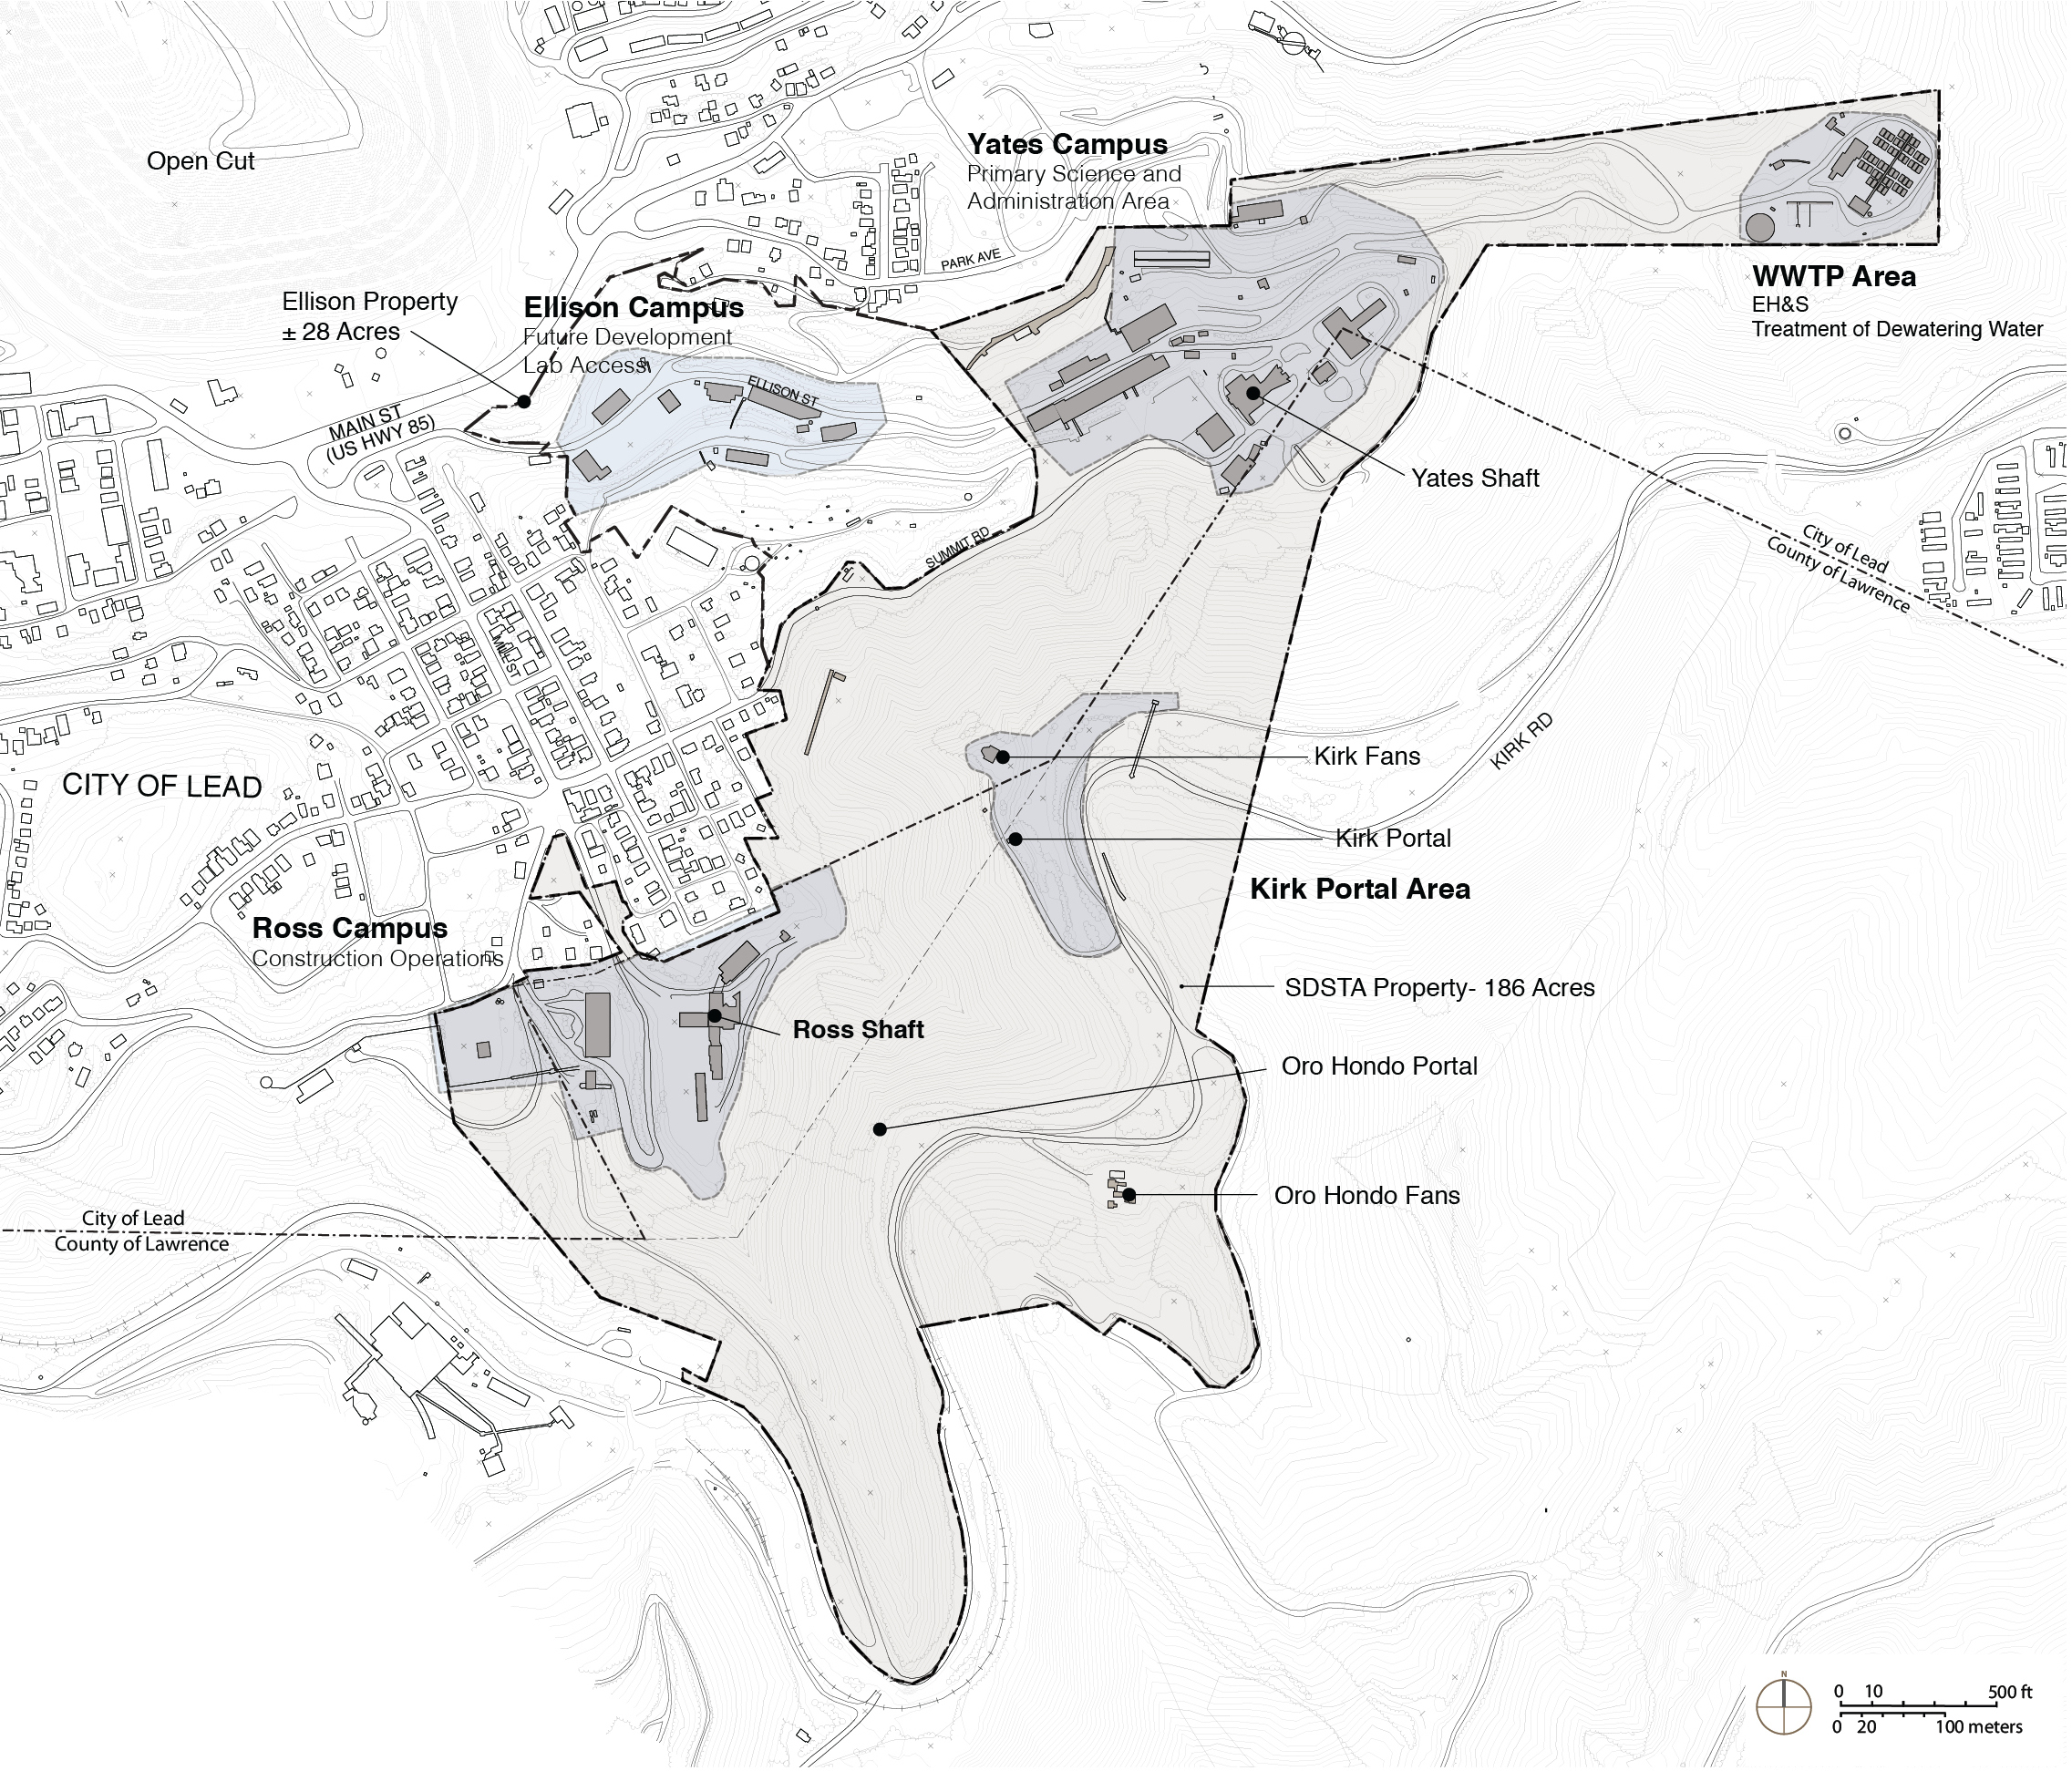
\includegraphics[width=0.8\textwidth]{archit-site-plan}
\end{cdrfigure}

\begin{cdrfigure}[Ross Complex architectural site plan]{ross-archit-site-plan}{Ross Complex architectural site plan (Arup)}
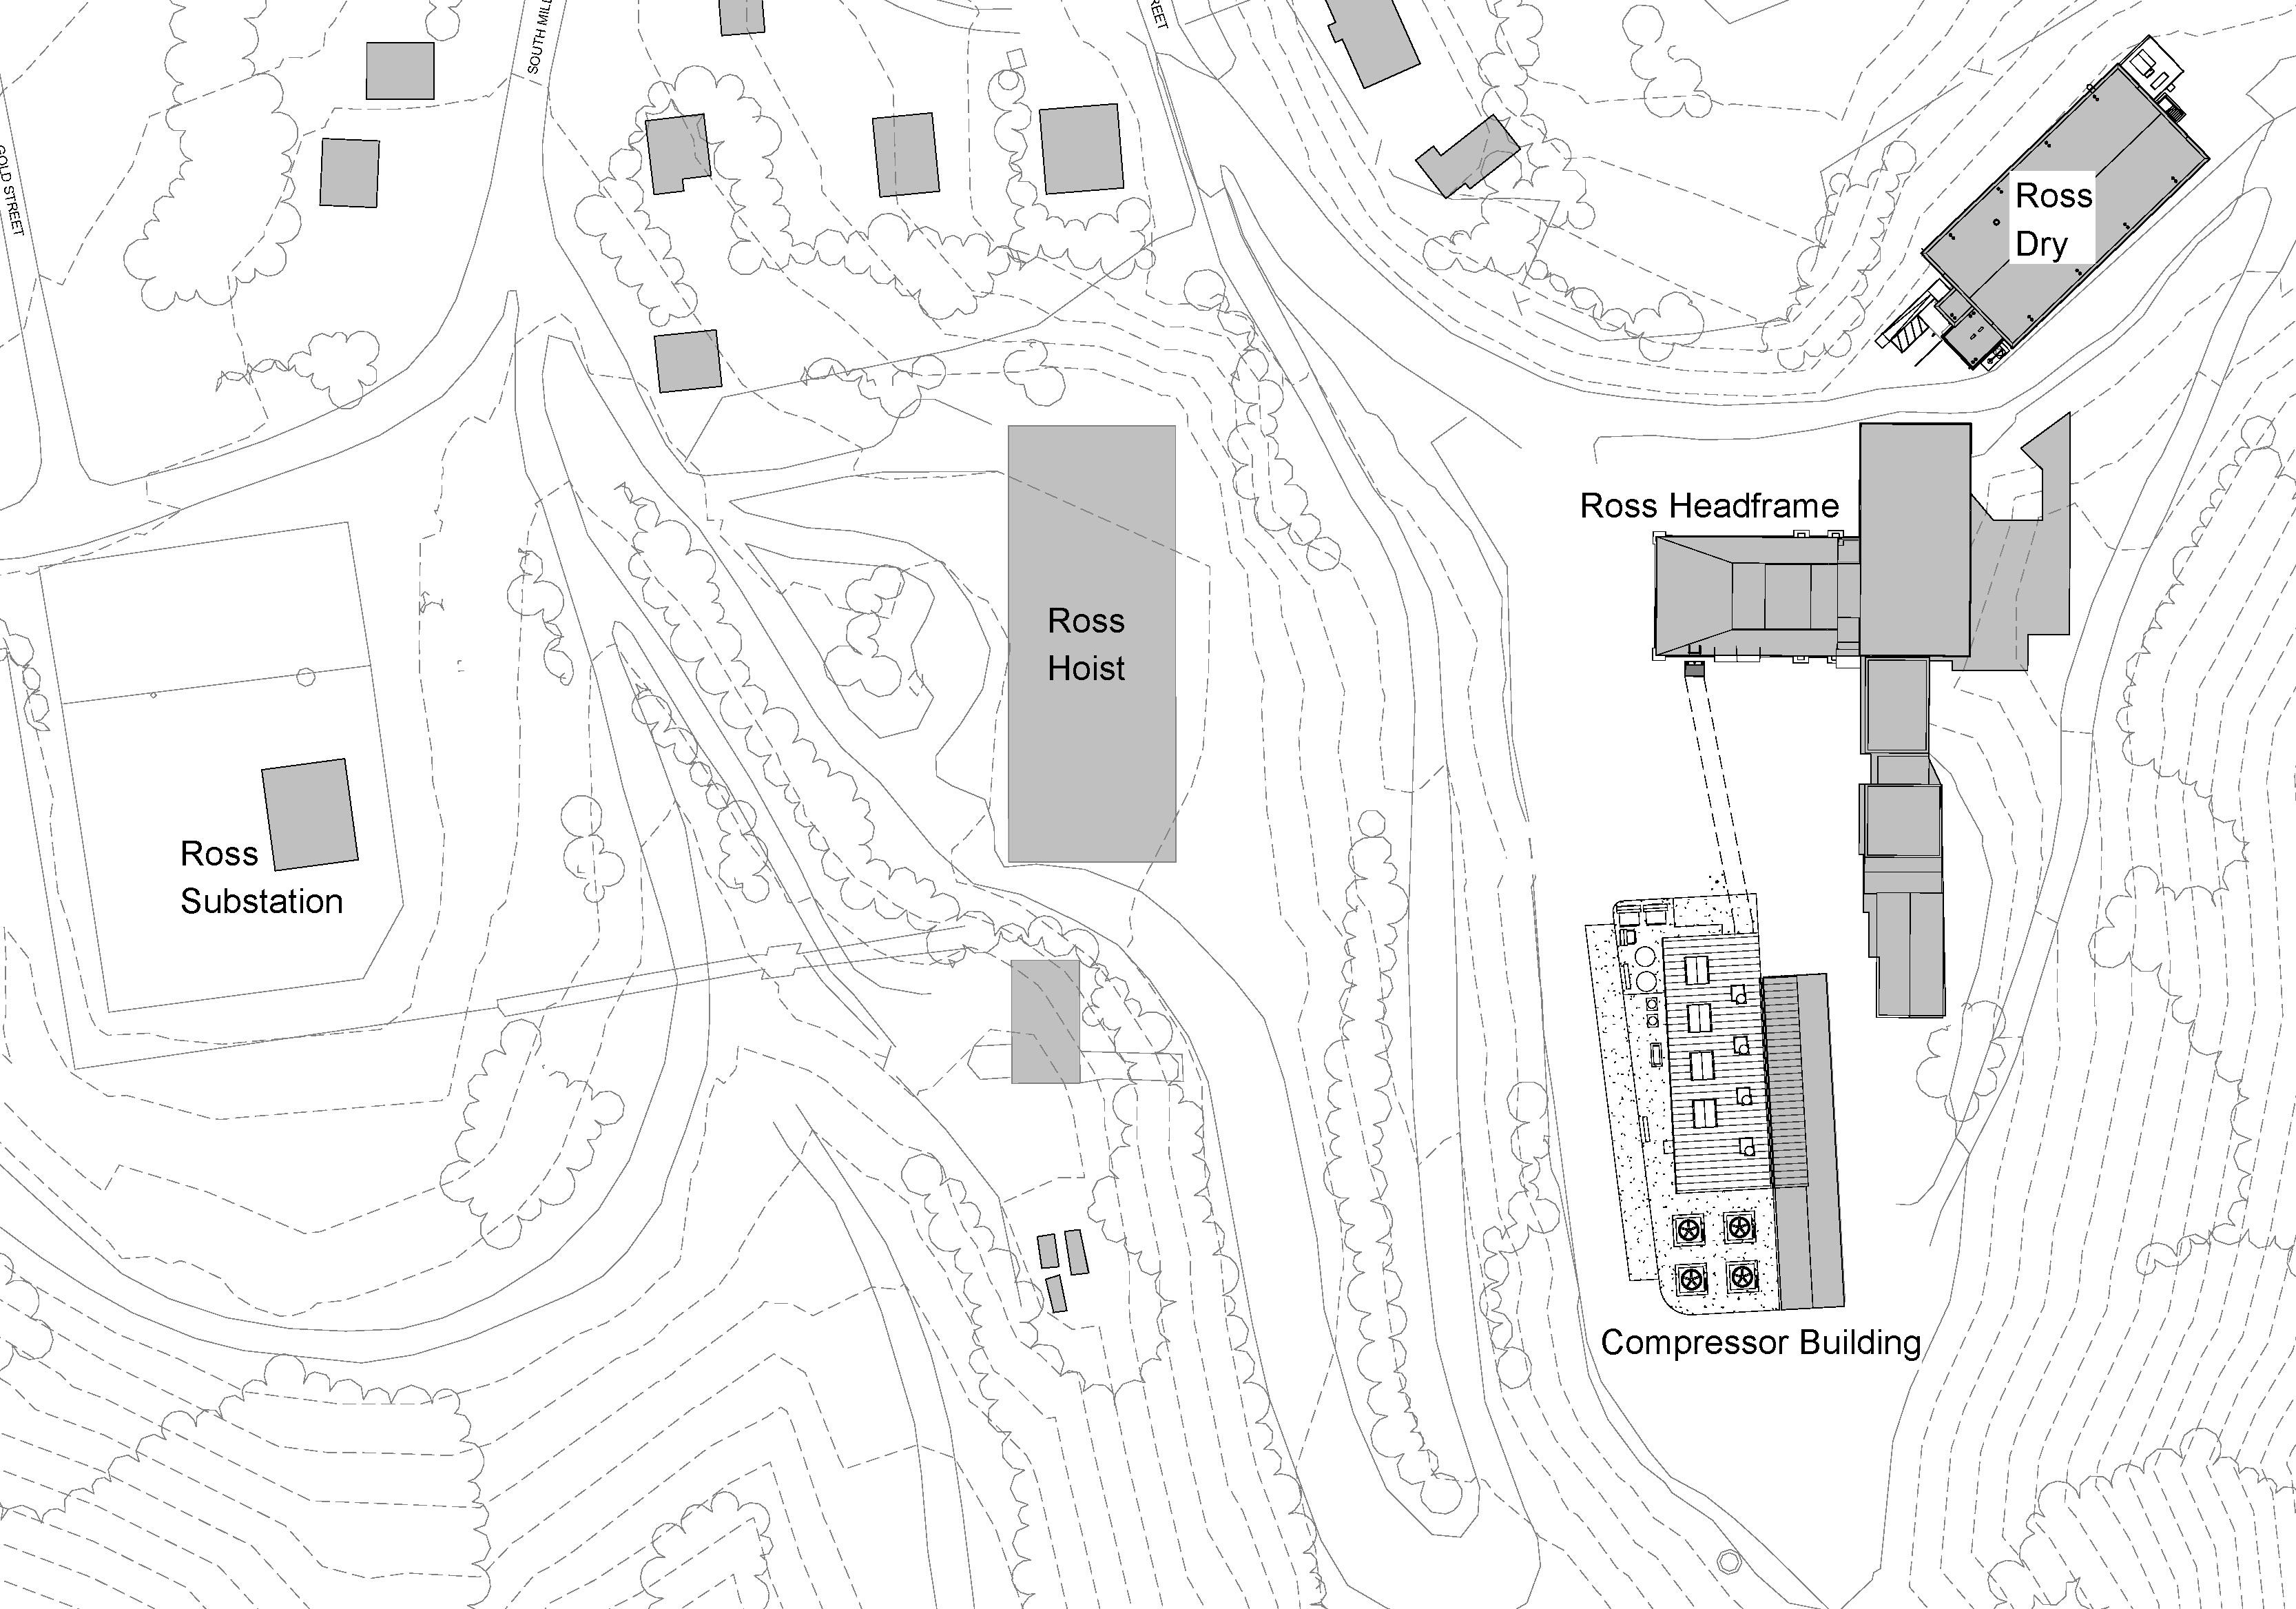
\includegraphics[width=\textwidth]{ross-archit-site-plan}
\end{cdrfigure}

%%%%%%%%%%%%%%%%%%%%%%%%%%%%%%%%%%%%%%%%%%%%%%%%%%%%%%%%%%%%%%%%%%%
\section{Surface Buildings}
\label{sec:fscf-surf-facil-surface-bldg}

Surface facilities utilized for the LBNF include those necessary for safe access and egress to the underground through the Ross Shaft, as well as spaces for offices. Existing buildings necessary for LBNF will be rehabilitated to code-compliance and to provide for the needs of the experiment. The only new building will be to provide space for compressors used to transfer cryogens from new receiving tanks on surface to the detectors underground. The existing Ross Dry building will be modified to provide space for a surface control room and offices. Much of the text below is excerpted from the 100\% Preliminary Design Report [12] provided by Arup, USA.

A new building and surrounding concrete slabs are planned to provide space for equipment to allow conversion of liquid argon and liquid nitrogen to gaseous form and compression of the nitrogen for delivery through the shaft to the underground where they are returned to liquid form as described later in this PDR in Chapter 4. \fixme{I don't find this; probably described in cryo annex} The location of this building was selected based on proximity to the shaft and truck accessibility, as thousands of truckloads of argon are required to fill the detectors underground.

In addition to housing nitrogen compressors inside the building, concrete slabs are provided around the building to allow for installation of argon and nitrogen receiving dewars for truck unloading, vaporizers to boil the liquids into gas, and electrical transformer to supply power to the (4) 1,500 Hp compressors, a standby generator, and cooling towers to reject heat generated through compression. All equipment except the cooling towers and associated circulation pumps is provided by the Cryogenics Infrastructure Project. The architectural layout of this building and surrounding equipment is provided in Figure~\ref{fig:compressor-bldg}.

\begin{cdrfigure}[Architectural layout of LBNF Cryogenics Compressor Building]{compressor-bldg}{Architectural layout of LBNF Cryogenics Compressor Building}
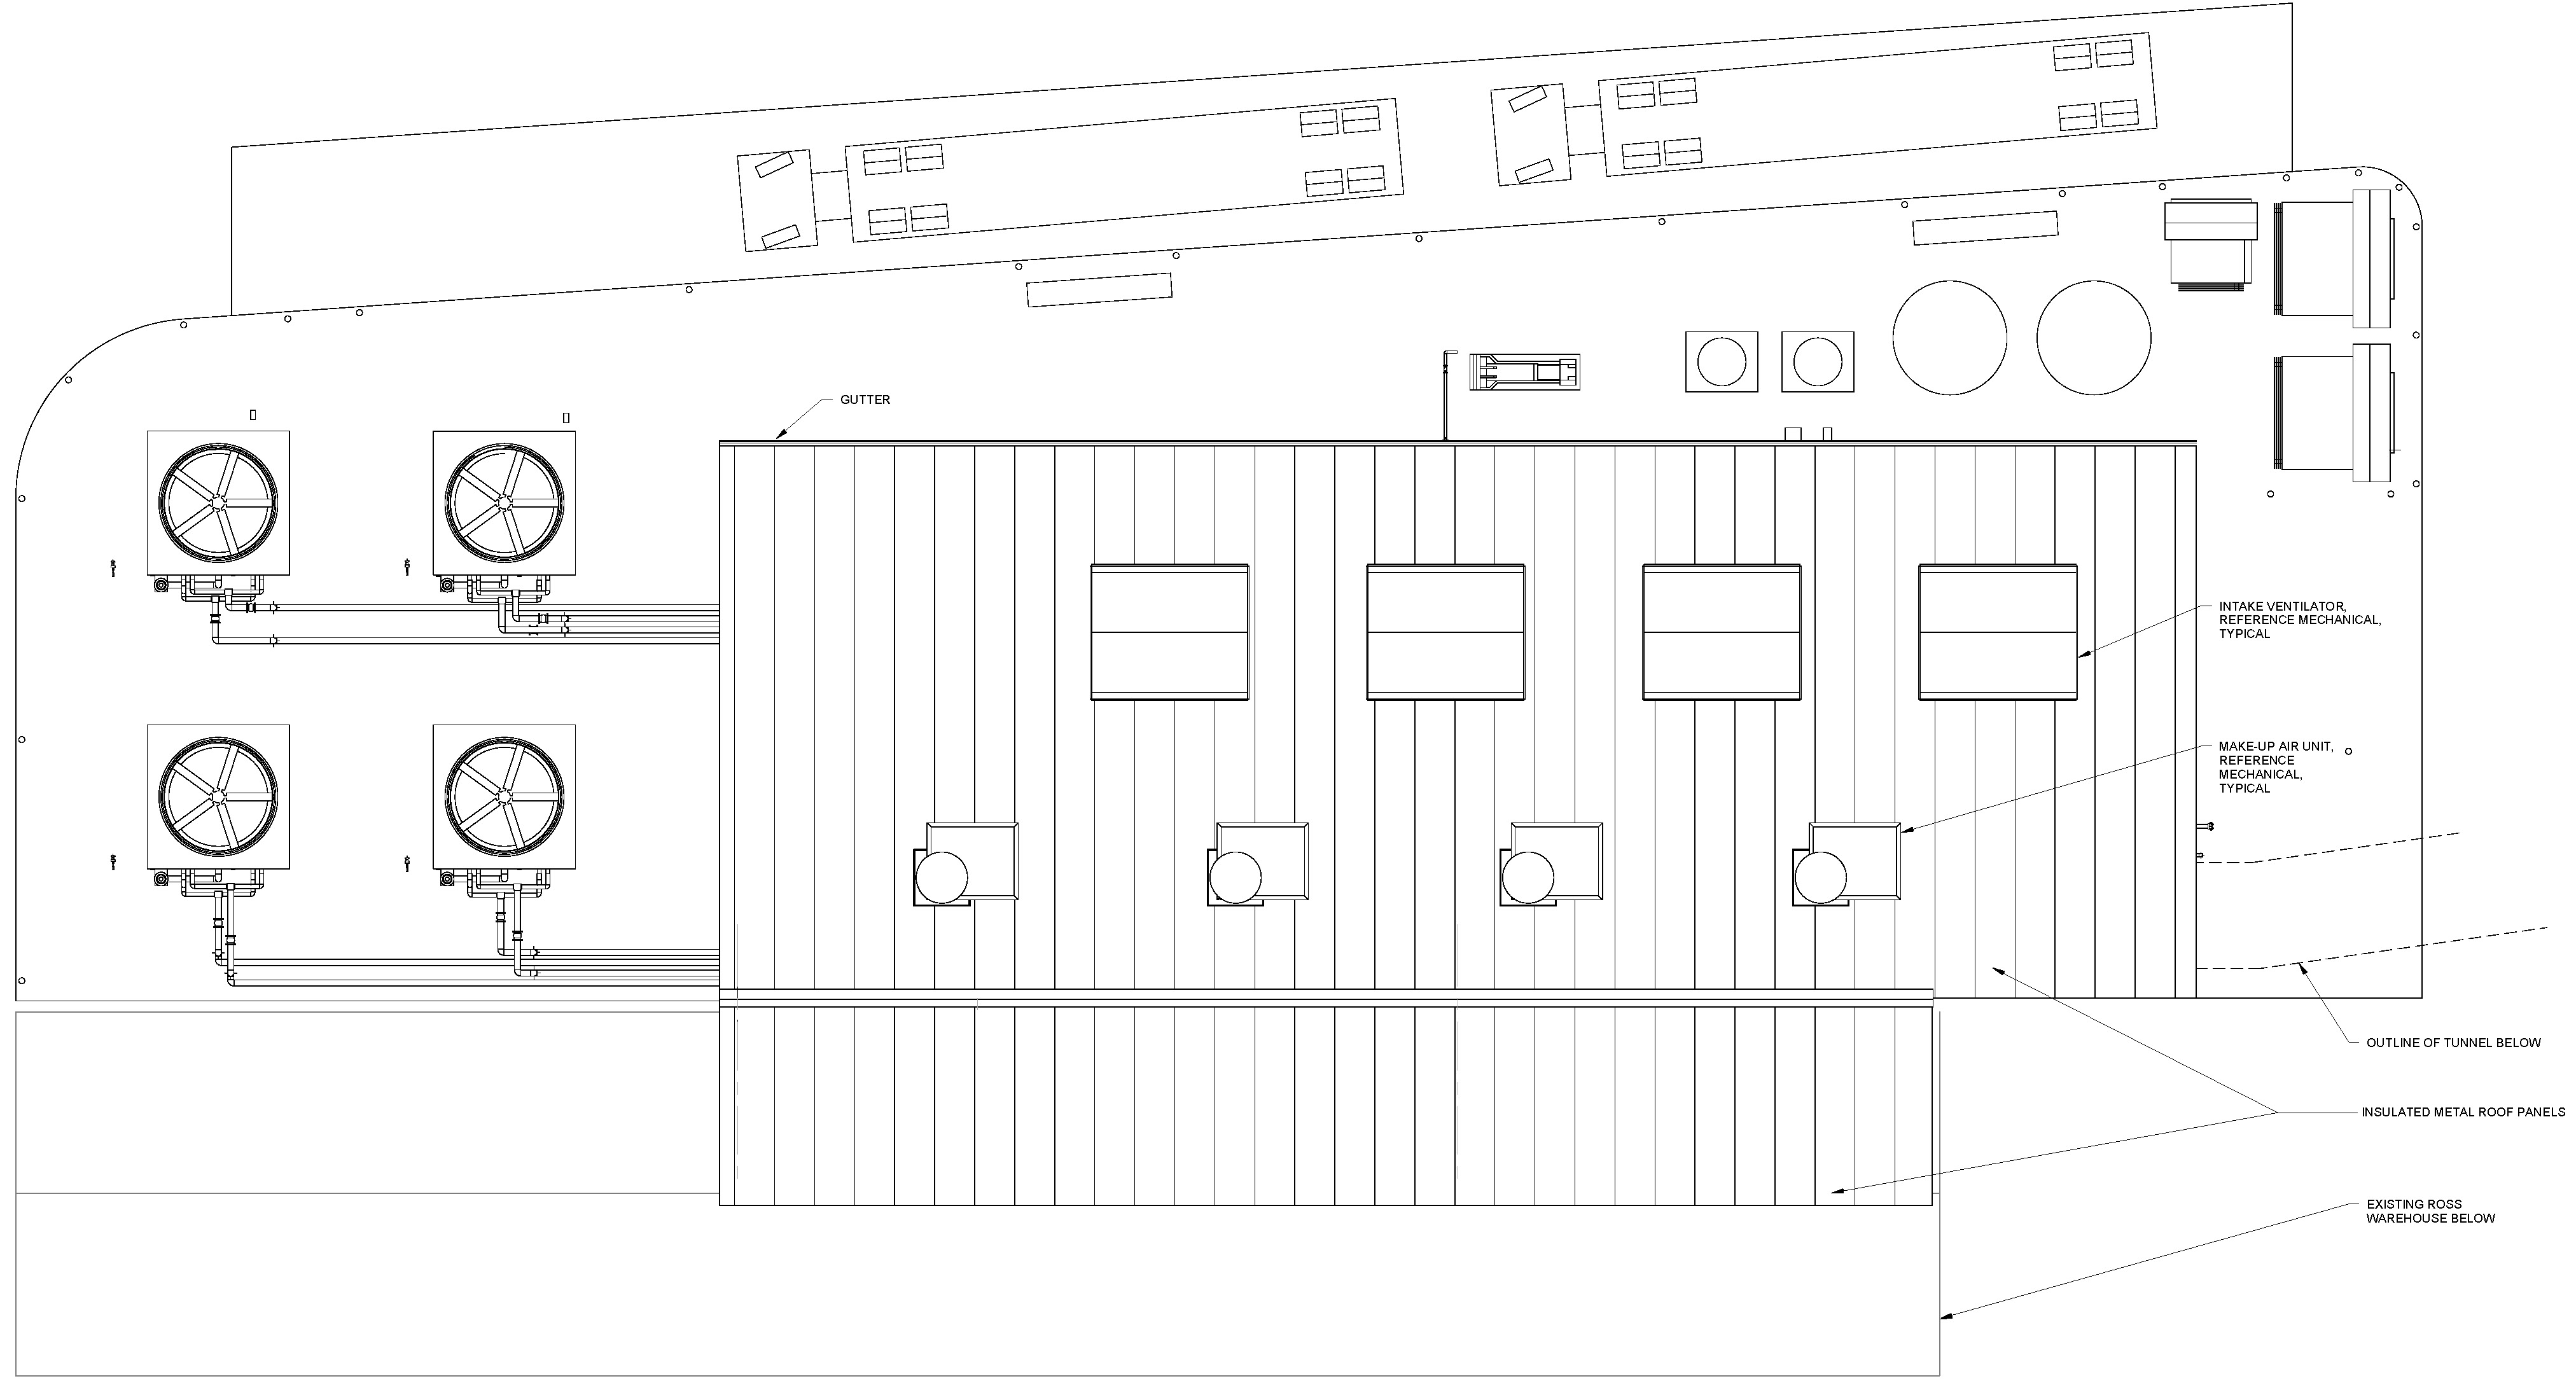
\includegraphics[width=\textwidth, angle=90]{compressor-bldg}
\end{cdrfigure}


%%%%%%%%%%%%%%%%%%%%%%%%%%%%%%%%%%
\subsection{Ross Dry}
\label{sec:fscf-surf-facil-surface-bldg-rossdry}

The Ross Dry building is in use by SURF to provide office and meeting space in addition to men's and women's dry facilities and emergency response capabilities. As a scope option, the design has included a complete renovation of this building to upgrade those existing capabilities and add space for an above-ground control room.  The control room itself is not a scope option, but all other refurbishment is.  This design includes flexible space that can be tailored to individual user's needs as the project transitions from construction through operations. 

The exterior of the Ross Dry is shown in Figure~\ref{fig:ross-dry-ext}. The renovations of this building are shown in Figures~\ref{fig:cmd-control-center-main} and~\ref{fig:cmd-control-center-basement}.

\begin{cdrfigure}[Photo of Ross Dry exterior]{ross-dry-ext}{Photo of Ross Dry exterior (HDR) \fixme{Need orig; too fuzzy}}
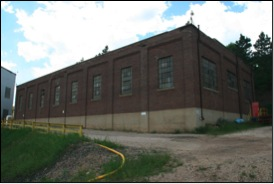
\includegraphics[width=0.8\textwidth]{ross-dry-ext}
\end{cdrfigure}

\begin{cdrfigure}[Ross Dry renovation, main floor.  The control room could be located in any office space, but is planned in the room at the bottom of this image.]{cmd-control-center-main}{Location of new Command and Control Center (SURF), main floor.}
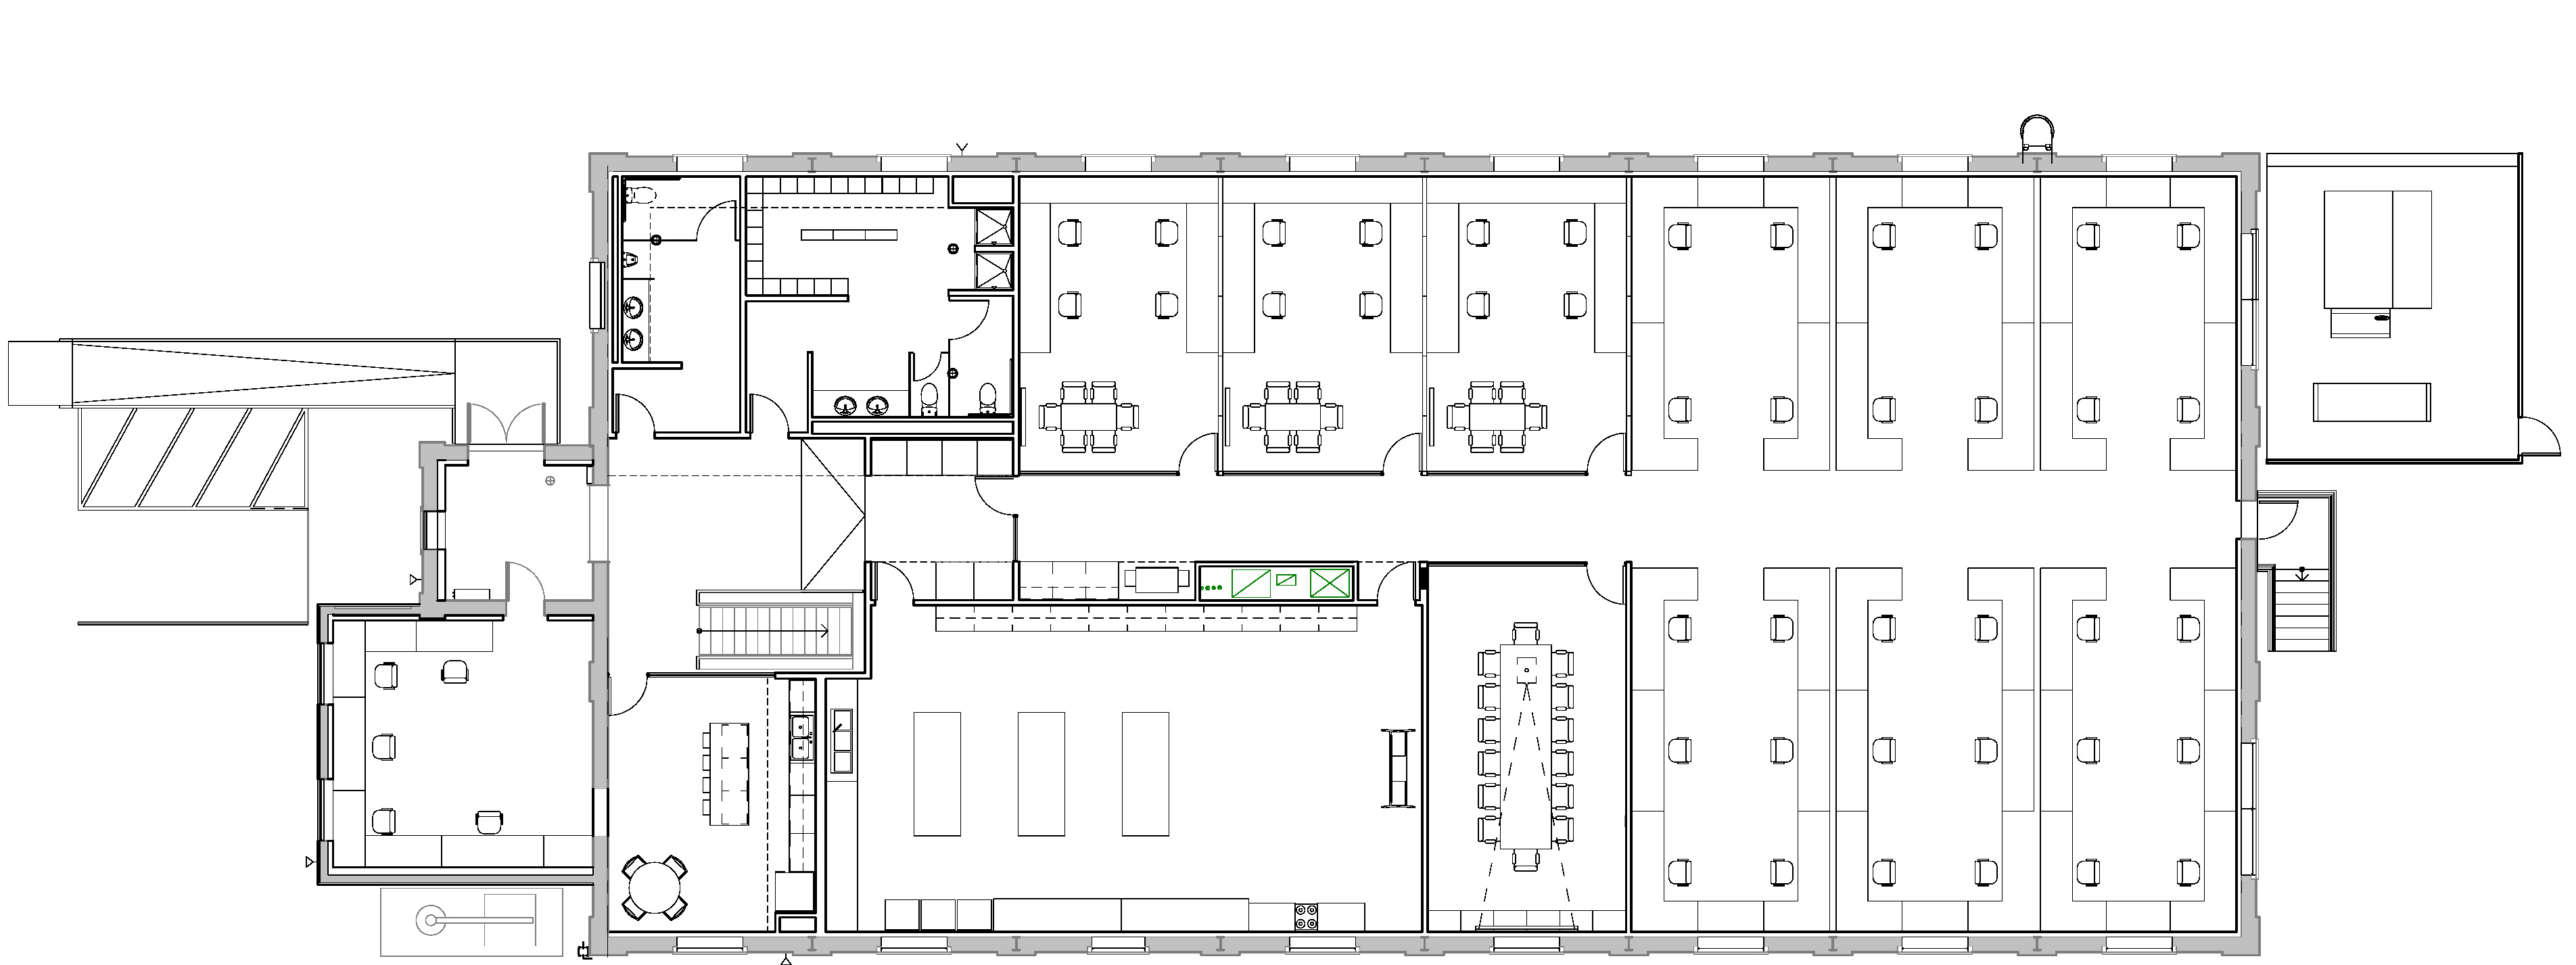
\includegraphics[width=\textwidth, angle=90]{ross-dry-building-main-floor}
\end{cdrfigure}

\begin{cdrfigure}[Ross Dry Renovation, basement]{cmd-control-center-basement}{Location of new Command and Control Center (SURF), basement.}
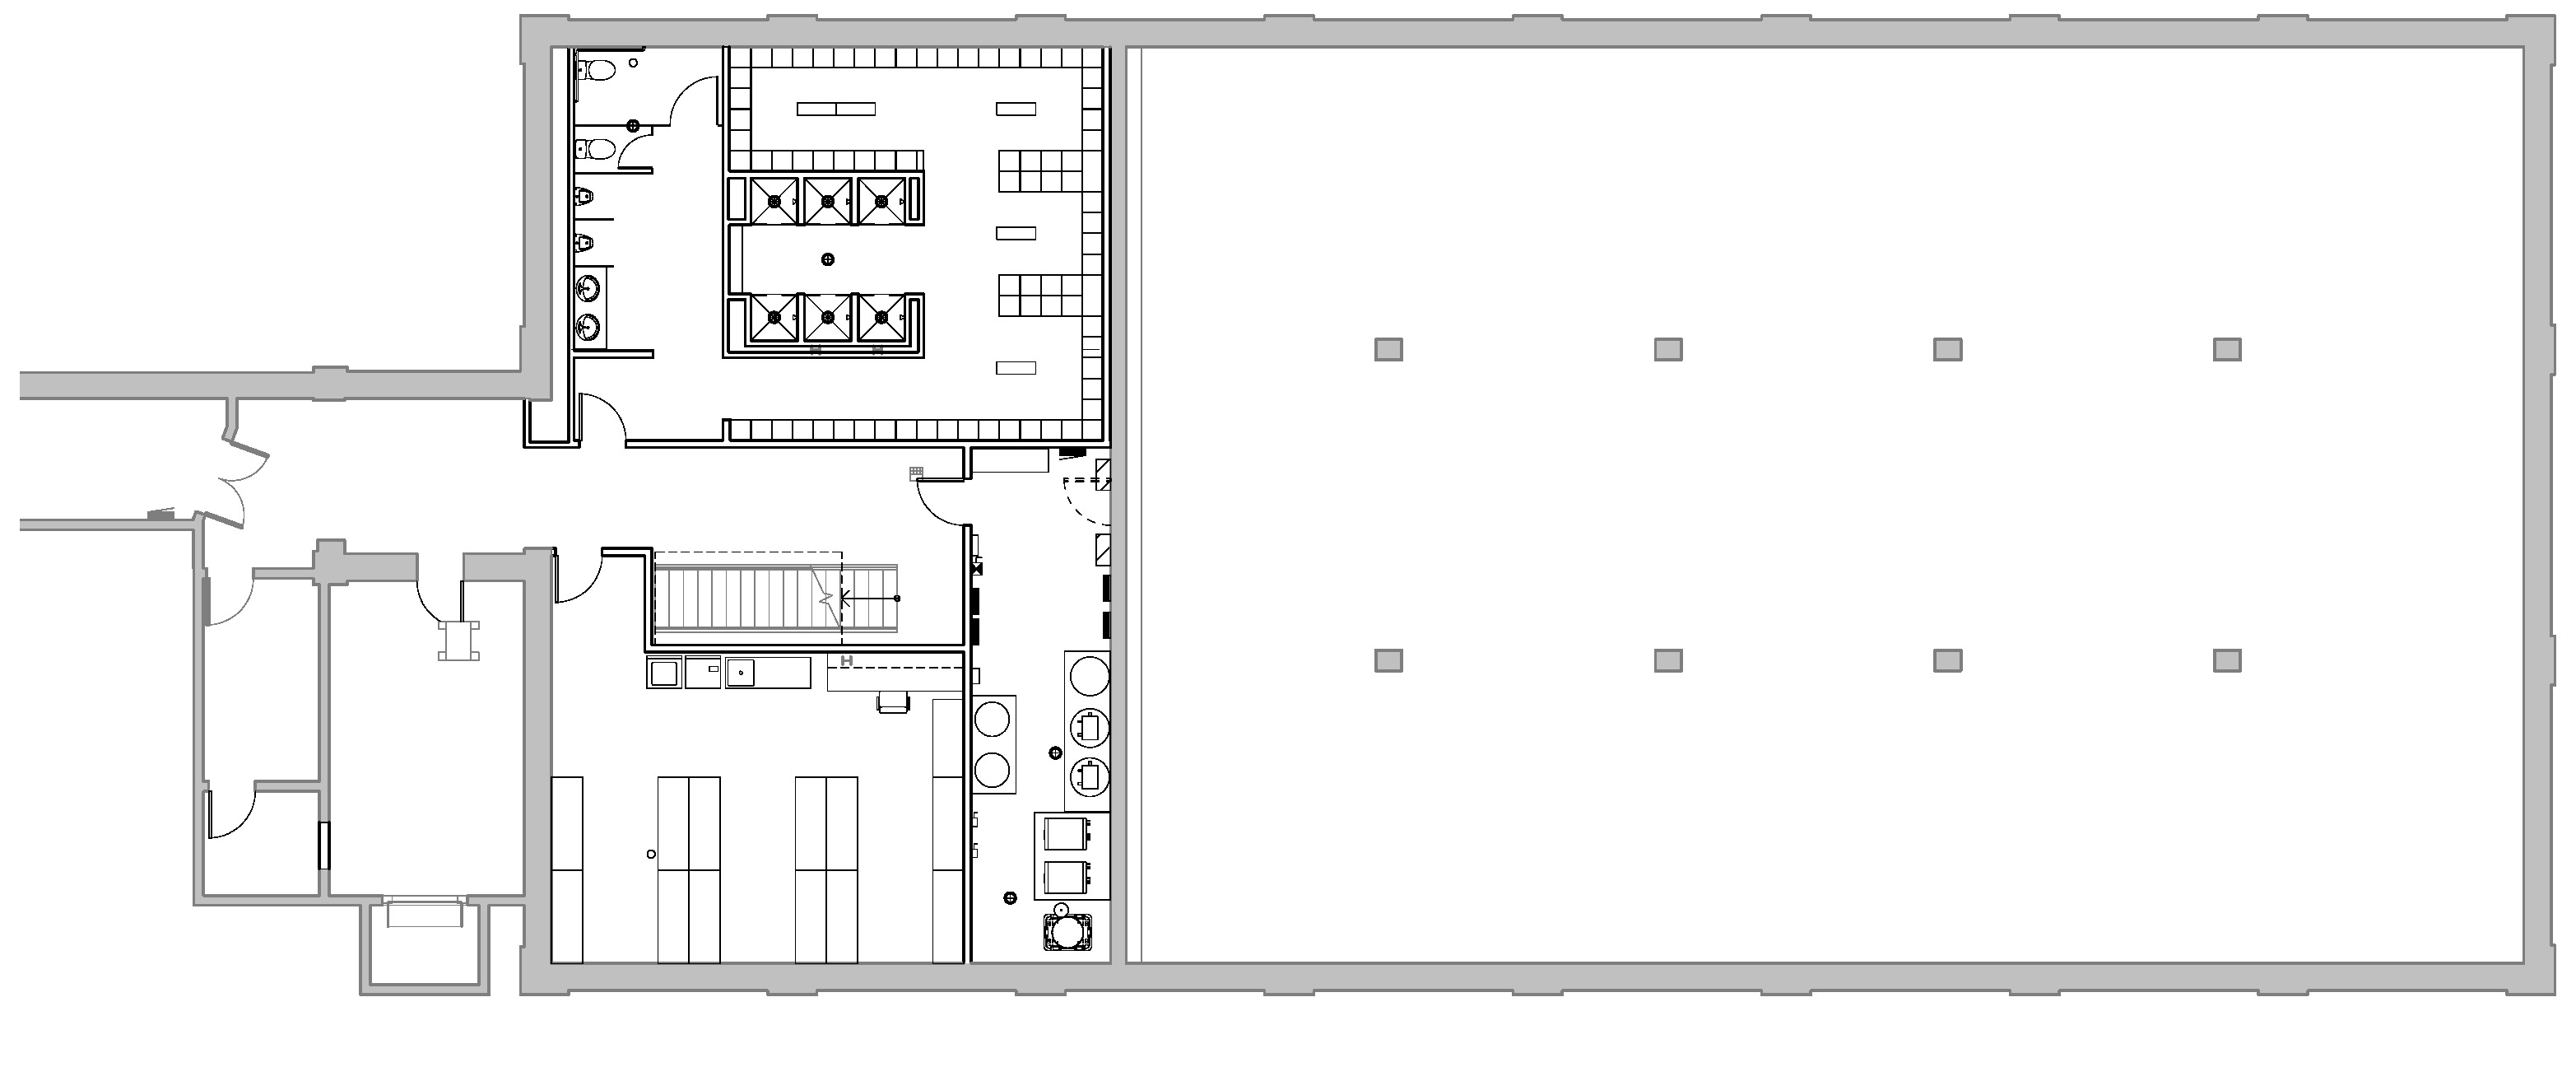
\includegraphics[width=\textwidth, angle=90]{ross-dry-building-basement}
\end{cdrfigure}


%%%%%%%%%%%%%%%%%%%%%%%%%%%%%%%%%%
\subsection{Ross Headframe and Hoist Buildings}
\label{sec:fscf-surf-facil-surface-bldg-rosshead}

The headframe and hoist buildings at the Ross Campus provide services for LBNF use. The Ross Headframe Building will be the main entry point for construction activities as well as the ongoing operations and maintenance functions. Gas pipe from the LBNF Cryogenics Compressor Building will pass through this building to get to the shaft.

Following shaft rehabilitation, the LBNF project will include structural reinforcement of the Ross Headframe to meet current codes and standards.  The headframe will also be modified somewhat to accommodate longer loads than are currently possible.  This project will occur concurrently with other site preparation activities planned to be performed outside of the CD3a scope, as described in section \fixme{add link to new section on site preparation activities per Elaine�s request}


%%%%%%%%%%%%%%%%%%%%%%%%%%%%%%%%%%
\subsection{Yates Headframe Building}
\label{sec:fscf-surf-facil-surface-bldg-yateshead}\fixme {JCW - I just duplicated the title from above}

The headframe at the Yates Campus provide services for LBNF use. One scope option is to provide a redundant fiber optic backbone through this shaft, and the shaft will be used for delivery of people and materials for construction and operation of LBNF.  One specific time frame where this shaft will be critical is during the installation of gas piping through the Ross shaft, during which time no other uses beyond emergency egress are possible.  Due to this demand, the LBNF project will include structural reinforcement of the Yates Headframe to meet current codes and standards.  This project will be completed prior to the installation of gas piping through the Ross shaft to ensure reliable operation during that time.

%%%%%%%%%%%%%%%%%%%%%%%%%%%%%%%%%%
\subsection{Ross Crusher Building}
\label{sec:fscf-surf-facil-surface-bldg-rosscrusher}

The existing Ross Crusher Building is a high bay space that contains rock crushing equipment that will be used for construction operations. The exterior of the building will be repaired to create a warm, usable shell. The upgrade of the existing crusher equipment is part of the waste rock handling work scope (see Section~\ref{sec:fscf-und-waste-rock}) and not part of the building rehabilitation. 

%%%%%%%%%%%%%%%%%%%%%%%%%%%%%%%%%%%%%%%%%%%%%%%%%%%%%%%%%%%%%%%%%%%
\section{New Surface Infrastructure}
\label{sec:fscf-surf-facil-surface-new}

Surface infrastructure includes surface structures such as retaining walls and parking lots, as well as utilities to service both buildings and underground areas. Existing infrastructure requires both rehabilitation as well as upgrading to meet code requirements and LBNF needs. The experiment needs were documented in the requirements found in LBNF Requirements Document\cite{dune-sci-req} and combined with facility needs for the design detailed in the Arup 100\% Preliminary Design Report\cite{arup:fscf100pdr}.

No new roads or parking lots are required for LBNF at SURF. The Ross Complex site will require minor demolition of power lines and a fire hydrant that are no longer used to provide adequate accessibility for truck traffic to the new Cryogenics Compressor Building. An existing space will be designated for handicap parking adjacent to the Ross Dry Building. Additional road work is required for truck transportation of waste rock, as described in the waste rock handling section.




